\documentclass{article}
\usepackage{graphicx}


\author{Martinez, Luis E\\
		Janicke, Marla\\
		Zhanaidarova, Maiya}
\title{Ex 4.3}		
\begin{document}
\maketitle
The solution is in the folder \textbf{ex4-3}, where there is  a \textbf{README.md} file with instructions to run it. We made the different meshes in Gmsh.app for a range of meshes running the command on the terminal \textbf{gmsh cube.geo -3  -clscale 0.5  -o cube.msh}, this example if for mesh size of $0.5$ for the dimension $3$. and we got the messhes as \ref{fig:2dmesh} and \ref{fig:3dmesh}.
\begin{figure}
	\centering
	\includegraphics[width =9cm]{mesh2d.png}
	\caption{the mesh for a size of $0.2$}
	\label{fig:2dmesh}
\end{figure}
\begin{figure}
	\centering
	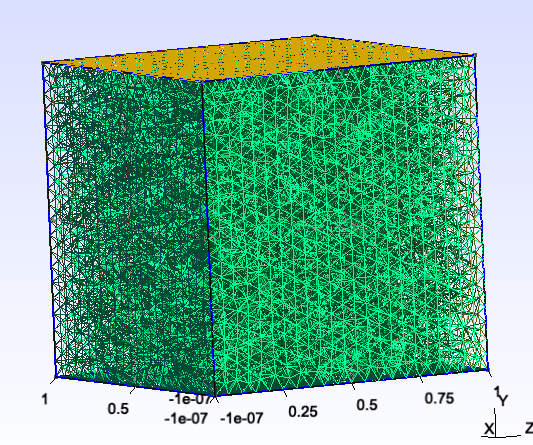
\includegraphics[width =9cm]{mesh3d.png}
	\caption{the mesh for a size of $0.2$}
	\label{fig:3dmesh}
\end{figure}

For $N=1$ we got the following table \ref{tab:1d}:
\begin{table}[h!]
  \begin{tabular}{rrrr}
    \hline\hline
    \textbf{mesh size} & \textbf{run-t Sparse} & \textbf{run-t Dense } & \textbf{diference time} \\ \hline
    5.00e-01 & 0.00 & 5.95e-06 & 0.00 \\
    4.00e-01 & 0.00 & 4.96e-06 & 0.00 \\
    3.00e-01 & 0.00 & 8.92e-06 & 0.00 \\
    2.00e-01 & 0.00 & 8.33e-06 & 0.00 \\ \hline\hline
  \end{tabular}
  \label{tab:1d}
\end{table}\\
for the case of 2 dimentions
\begin{table}[h!]
  \begin{tabular}{rrrr}
    \hline\hline
    \textbf{mesh size} & \textbf{run-t Sparse} & \textbf{run-t Dense} & \textbf{diference time} \\\hline
    1.00e+00 & 0.00 & 6.19e-05 & 0.00 \\
    5.00e-01 & 0.00 & 7.53e-04 & 0.00 \\
    3.00e-01 & 0.00 & 6.71e-03 & 0.01 \\
    2.00e-01 & 0.00 & 4.64e-02 & 0.04 \\\hline\hline
  \end{tabular}
\end{table}\\
and for 3 dimentions 
\begin{table}[h!]
  \begin{tabular}{rrrr}
    \hline\hline
    \textbf{mesh size} & \textbf{run-t Sparse} & \textbf{run-t Dense} & \textbf{diference time} \\\hline
    1.00e+00 & 0.00 & 9.37e-04 & 0.00 \\
    5.00e-01 & 0.01 & 7.49e-02 & 0.07 \\
    3.00e-01 & 0.05 & 2.96e+00 & 2.91 \\
    2.00e-01 & 0.33 & 7.55e+01 & 75.18 \\\hline\hline
  \end{tabular}
\end{table}\\
As we can observe the time grows too much in the mesh size from $0.3$ to $0.2$ in the order of minutes, so we can observe the inefficiency of dense matrix.\\
\textbf{note:} for smaller meshes than 0.2 the kernel restar several times, so we didn't include a finer mesh.
\end{document}